\section{Introduction}
\setcounter{page}{1}
\pagenumbering{arabic}


In this project we are going to find the optimal path for a solar powered airplane \footnote{Like the one from \url{http://www.solarimpulse.com/}}. During flight the plane's electrical engines drain power from it's battery, while at the same time solar panels on the plane's wings convert energy from the sun's rays into electric energy. However clouds may block the sun's rays from reaching the panels. In addition the sun's intensity increases when flying closer to the equator. In order to keep as much energy in the batteries as possible the flight path has to be optimized.

In this paper we will start by explaining the mathematical parameters we have taken into count to calculate the optimal path.
Afterwards we will formulate the problem in it's standard form.
We will finish by presenting some of the results obtained by the optimisation.


\subsection{Formulation of the problem.}

The main goal of this project is to find the best path connecting the starting point of the plane to the destination.
Before this question can be answered we first have to define what we mean by the best path.
We could for instance look at the shortest path, the most sunny path, the fastest path, \dots 
A logical choice to make was to define the best path as the path that yielded the most energy, at the end of the flight.

To calculate this energy we have taken several parameters in to account like the solar energy, the drag force on the plane and the cost for accelerating the plane.
The combinations of the energy losses and gains will be combined to calculate the best path.
Next we will give a brief explanation about all of these parameters and their mathematical formulation.

\subsubsection{Solar energy}

The solar gain is roughly defined as how much sun we can pick up in our flight path.
The local amount of sun is determined by two factors, the angle of the sun at that time and that place and the local cloud density.

For the inclination angle of the sun we used \textbf{\dots}

To simulate clouds we where looking for highly autocorrelated random data so that the clouds would be located in islands rather than being scattered without any pattern in the sky.
The technique we applied was to generate a low dimensional matrix random matrix and extrapolate the data points to get a continuous grid.
An example of the simulated weather is shown in Figure \ref{fig:RandomWeather}.

At the end the local solar gain is eventually calculated by the product of the suns intensity and the amount of clouds.
\begin{equation}
E_{sun}(x,y)  =  V_{sun}(x,y) V_{Cloud}(x,y)
\end{equation}
The total amount of energy collected by the airplane is now given by 
\begin{equation}
E_{sun}(t)  =  -\alpha_{sun}\oint_{path} E_{sun}(x,y)  d\tau,
\end{equation}
this path integral is evaluated over the path from $ \tau=0 $ till $ \tau=t $.
The constant term in front of the integral is a scaling term that can be adjusted to tune the weight of the individual energies.
Remark the minus sing in front of the integral, this implies that we want to maximise the solar gain.



\begin{figure}
\centering
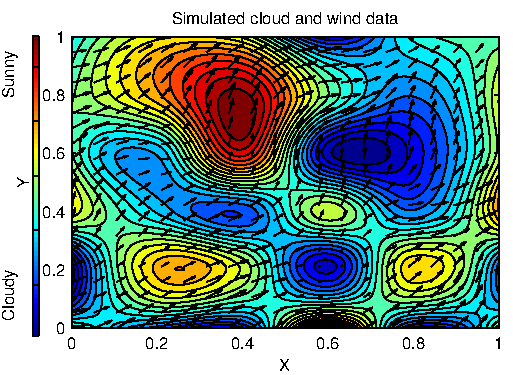
\includegraphics[width=0.5\linewidth]{../src/plot/RandomWeather}
\caption{An example of  simulated weather data. The colour map represents the intensity of the sun, the arrows point in the direction of the wind. This data is created by the  interpolation on a 4 by 4 random generated matrix. }
\label{fig:RandomWeather}
\end{figure}


\subsubsection{Drag resistance}

A second import aspect that influences the energy balance of the airplane is the drag force.
The introducing a drag force will keep the velocity of the plane bounded.
We chose to use a simple quadratic dependency of the the drag force and the speed.
The drag force is then defined as 
\begin{equation}
E_{drag}(t)  =  \alpha_{drag} \oint_{path} v(x,y).^2  d \tau,
\end{equation}
the same conventions for the integral apply as noted above.


\subsubsection{Acceleration force}

The acceleration force is the last parameter that we looked at.





